% Distributed under the MIT License.
% (See accompanying file LICENSE.txt)
% (C) Copyright NoWork team

\documentclass[12pt,a4paper]{article}

\usepackage[utf8]{inputenc}
\usepackage[french]{babel}
\usepackage[T1]{fontenc}
\usepackage{verbatim}
\usepackage{graphicx}
\usepackage{listings}

\title{NoWork\\
Analyse du cahier des charges}
\author{Équipe de développement NoWork\\[2em]}
\date\today

\newcommand{\latex}{\LaTeX\space}

\begin{document}
\maketitle

\section{Introduction}

Ce document analyse le cahier des charges initialement décrit par M. Frédéric Peschanski qui nous a été remis le 6 novembre 2013. L'objectif de ce travail est d'étudier les systèmes de réécriture afin de développer un logiciel permettant la réécriture de terme suivant une stratégie.

\section{Infrastructure technique}

\subsection{Dépendances}

\begin{itemize}
\item Compilateur OCaml 4.00.1 et la librairie standard OCaml ;
\item Le moteur de production \textit{GNU make} ;
\item Le moteur de production et de test \textit{ocp-build} version 1.99 ;
\item Le gestionnaire de paquet \textit{opam} version 1.1.0 ;
\item Le gestionnaire de version git.
\end{itemize}
\vspace{10pt}

Il n'y a pas de version web disponible donc il n'y a pas de dépendance vers \textit{js-of-ocaml}.

\subsection{Guide de style}

Le guide de style a été développé avec le client et est disponible en \latex dans le répertoire \verb=doc/coding-style.tex=. La documentation a été rédigée en \textit{OCamlDoc} et est disponible dans le répertoire \verb=doc/reference/=.

\subsection{Tests}

Le code est testé et les tests fonctionnels sont directement embarqués dans le langage. Les utilisateurs pourront donc eux-mêmes tester le code qu'ils auront écrit. Le répertoire \verb=data/test/= contient tous nos fichiers de tests et se décline en deux sous-dossiers \verb=run-fail/= et \verb=run-pass=, le premier contenant les fichiers testant les erreurs devant être déclenchées, et le deuxième testant qu'aucune erreur n'est lancée. Les tests unitaires sont réalisés dans le dossier \verb=tests/= et \textit{ocp-build} est utilisé pour déclencher ces tests.

\subsection{Organisation du projet}

Le cahier des charges initial spécifiait un module différent pour la représentation des termes et du système or il s'est avéré que les deux étaient trop fortement couplé et que des simplifications au niveau du code impliquait ses deux modules d'être unifié. Pour rappel, les modules sont :

\begin{itemize}
\item Module d'analyse lexicale et syntaxique (\verb=src/parser/=) ;
\item Module de représentation du système de réécriture et des termes (\verb=src/system/=) ;
\item Module de gestion du simulateur (\verb=src/algorithm=) ;
\item Module pour le \textit{top-level} (\verb=src/interactive=) ;
\item Module pour les tests unitaires (\verb=tests/=).
\end{itemize}

Il n'y a pas de module de gestion de l'exploration car cette fonctionnalité n'a pas été implémentée.

\section{Fonctionnalités}

La liste de functionalites est montre dans le diagram de cas
d'utilisation de la figure~\ref{use-cases}. A continuation vous
pouvais trouver une description de chacun des cas d'utilitation avec
des examples:

\begin{figure}[h!]
  \centering
  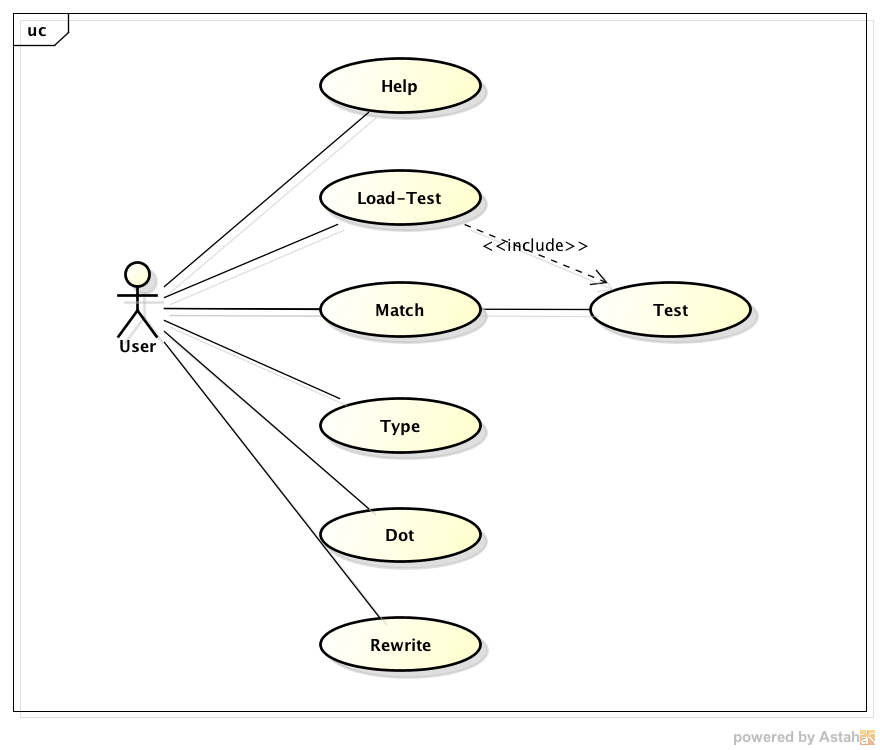
\includegraphics[width=\linewidth,natwidth=\linewidth,natheight=\textheight]{use-case-diagram.png}
  \caption{List of use cases for nowork}
  \label{use-cases}
\end{figure}

\begin{description}

\item[Help:]
Montre une liste de command disponible avec une description des chacun
des options.

\begin{minipage}{\textwidth}
Result:
\begin{lstlisting}[breaklines=true,basicstyle=\ttfamily\footnotesize]
Available commands :
        :help            -- Displays this help
        :?               -- Displays this help
        :load-test f exp -- Load a test file f and check that the result matches the expectation
        :test            -- Test an expression (consult user-doc for more infos)
        :match           -- Check that an expression matches the given type or strategy
        :type            -- Returns the type of the expression
        :dot t out       -- Output the hash-consed version of a term into a dot file graph
        :quit            -- Exits the REPL
        :exit            -- Exits the REPL
        :q               -- Exits the REPL
More detailled informations may be found in the user-documentation
\end{lstlisting}
\end{minipage}

\item[Load-test:]
Permet de charger un fichier de text l'executer et verifier le resultat que on
doit s'attendre. Le test passe si le resultat de l'execution
correspond avec le resultat attendu. \\

\begin{minipage}{\textwidth}
Example :
\begin{lstlisting}[breaklines=true,basicstyle=\ttfamily\footnotesize]
  # :load-test "data/test/run-fail/typecheck_unification2.nw" --failwith RewritingSystemError.TypeClash ;;
    Filename: data/test/run-fail/typecheck_unification2.nw
    [ passed ]  Failure with RewritingSystemError.TypeClash as expected.
        Info: Type clash between A and K2.
\end{lstlisting}
\end{minipage}

\item[Test:]
Permet de tester une terme ecrit dans la ligne des commandes.\\

 \begin{minipage}{\textwidth}
Example :
\begin{lstlisting}[breaklines=true,basicstyle=\ttfamily\footnotesize]
  # :test  --failwith RewritingSystemError.TypeClash ;;
  Terms : Lambda (x, Var (x)) rewrote into :Lambda (x, Var (x))
[ passed ]  Terms have been correctly rewritten in : Lambda (x, Var (x));;
\end{lstlisting}
\end{minipage}

\item[Type:]
Permet d'obtenir le type de une terme ecrit dans la ligne des commandes.\\

\begin{minipage}{\textwidth}
Example :
\begin{lstlisting}[basicstyle=\ttfamily\footnotesize]
  # :type Lambda(x, Var(x));;
   Term
\end{lstlisting}
\end{minipage}

\item[Dot:]
Permet de generer un fichier dot avec la representation hash-conse
d'un term. \\

\begin{minipage}{\textwidth}
Example :
\begin{lstlisting}[basicstyle=\ttfamily\footnotesize]
  # :dot Lambda(x, Var(x)) "lambda.dot" ;;
\end{lstlisting}
\end{minipage}

\item[Match:]
Permet de voir si une term match un pattern donne. \\

\begin{minipage}{\textwidth}
Example :
\begin{lstlisting}[basicstyle=\ttfamily\footnotesize]
  # :match App(Lambda(x, Var(x)), Lambda(y, Var(y))) 
       --with App(?T, ?T)
\end{lstlisting}
\end{minipage}

\item[Quit:]
Arrete le program.

\end{description}

\end{document}

